\subsection{UC22 - Visualizzazione errore codice scaffalatura non valido}
\begin{figure}[H]
  \centering
  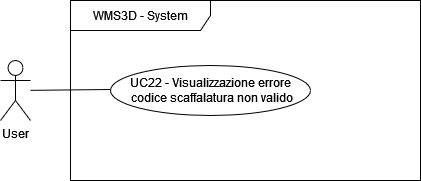
\includegraphics[width=0.8\textwidth]{UC_diagrams_21-26/UC22.drawio.png}
   \caption{Diagramma UML UC22}
\end{figure}
\begin{itemize}
    \item \textbf{Attori:} User.
    \item \textbf{Pre-condizione:}  L'utente ha inserito un codice identificativo di una scaffalatura che contiene caratteri invalidi oppure non è univoco.
    \item \textbf{Post-condizione:}  L'utente visualizza un messaggio d'errore e dovrà reinserire un codice diverso.
    \item \textbf{Scenario Principale:}  L'utente visualizza un messaggio informativo sull'errore e ne conferma la ricezione. L'operazione fallisce e l'utente dovrà scegliere un nuovo codice.
    \item \textbf{Generalizzazioni:} -
    \item \textbf{Estensioni:} -
\end{itemize}